%worksheet3.tex
%problem set for the course COMS10007 taught at the University of Bristol
%Conor Houghton conor.houghton@bristol.ac.uk

%To the extent possible under law, the author has dedicated all copyright 
%and related and neighboring rights to these notes to the public domain 
%worldwide. These notes are distributed without any warranty. 



\documentclass[11pt,a4paper]{scrartcl}
\typearea{12}
\usepackage{graphicx}
\usepackage{pstricks}
\usepackage{tikz-qtree}
\usepackage{listings}
\usepackage{color}
\usetikzlibrary{positioning}
\newif\ifanswers
\answerstrue
%\answersfalse

\lstset{language=C}
\pagestyle{headings}
\markright{COMS10001 - PandA2 algorithms worksheet 4 - Conor}
\begin{document}

\subsection*{Algorithms Worksheet 3}

This week there are two question each worth four marks, there are two
marks for attendance.

\begin{enumerate}

\item Us Dijkstra's algorithm to find the shortest path from $d$ to $c$ in
  \begin{center}
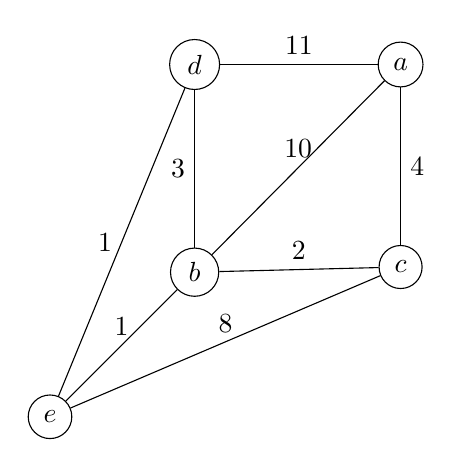
\begin{tikzpicture}
\node[draw,circle](a){$a$};
\node[draw,circle, below      =2cm of a](c){$c$};
\node[draw,circle, left = 2cm of a](d){$d$};
\node[draw,circle, below = 2 cm of d](b){$b$};
\node[draw,circle, below left = 2 cm of b](e){$e$};
\path (a) edge node[above]{10} (b);
\path (a) edge node[right]{4} (c);
\path (b) edge node[left]{3} (d);
\path (a) edge node[above]{11} (d);
\path (b) edge node[above]{2} (c);
\path (b) edge node[above]{1} (e);
\path (d) edge node[left]{1} (e);
\path (c) edge node[above]{8} (e);
\end{tikzpicture}
\end{center}

\ifanswers

\noindent Solution:

Set the distances as $\infty$ except the first node, the $x$ shows
there is no preceeding node.
\begin{center}
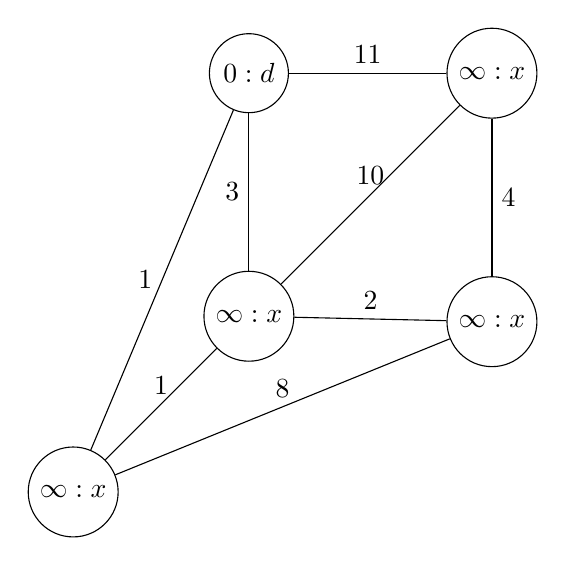
\begin{tikzpicture}
\node[draw,circle](a){$\infty:x$};
\node[draw,circle, below      =2cm of a](c){$\infty:x$};
\node[draw,circle, left = 2cm of a](d){$0:d$};
\node[draw,circle, below = 2 cm of d](b){$\infty:x$};
\node[draw,circle, below left = 2 cm of b](e){$\infty:x$};
\path (a) edge node[above]{10} (b);
\path (a) edge node[right]{4} (c);
\path (b) edge node[left]{3} (d);
\path (a) edge node[above]{11} (d);
\path (b) edge node[above]{2} (c);
\path (b) edge node[above]{1} (e);
\path (d) edge node[left]{1} (e);
\path (c) edge node[above]{8} (e);
\end{tikzpicture}
\end{center}
Update  the nodes adjacent to the starting node:
\begin{center}
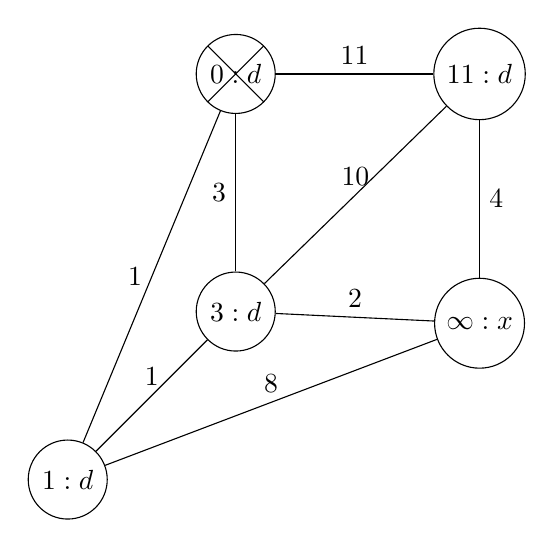
\begin{tikzpicture}
[cross/.style={path picture={ \draw[black] (path picture bounding
      box.south east) -- (path picture bounding box.north west) (path
      picture bounding box.south west) -- (path picture bounding
      box.north east); }}]
\node[draw,circle](a){$11:d$};
\node[draw,circle, below      =2cm of a](c){$\infty:x$};
\node[draw,circle,cross, left = 2cm of a](d){$0:d$};
\node[draw,circle, below = 2 cm of d](b){$3:d$};
\node[draw,circle, below left = 2 cm of b](e){$1:d$};
\path (a) edge node[above]{10} (b);
\path (a) edge node[right]{4} (c);
\path (b) edge node[left]{3} (d);
\path (a) edge node[above]{11} (d);
\path (b) edge node[above]{2} (c);
\path (b) edge node[above]{1} (e);
\path (d) edge node[left]{1} (e);
\path (c) edge node[above]{8} (e);
\end{tikzpicture}
\end{center}
Take the lowest distance node and update that:
\begin{center}
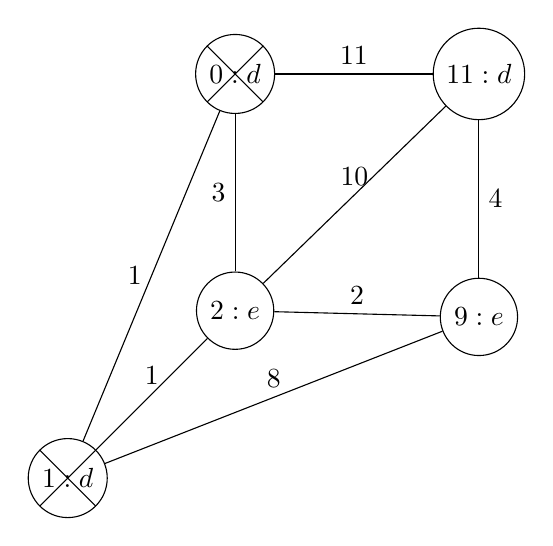
\begin{tikzpicture}
[cross/.style={path picture={ \draw[black] (path picture bounding
      box.south east) -- (path picture bounding box.north west) (path
      picture bounding box.south west) -- (path picture bounding
      box.north east); }}]
\node[draw,circle](a){$11:d$};
\node[draw,circle, below      =2cm of a](c){$9:e$};
\node[draw,circle,cross, left = 2cm of a](d){$0:d$};
\node[draw,circle, below = 2 cm of d](b){$2:e$};
\node[draw,circle,cross, below left = 2 cm of b](e){$1:d$};
\path (a) edge node[above]{10} (b);
\path (a) edge node[right]{4} (c);
\path (b) edge node[left]{3} (d);
\path (a) edge node[above]{11} (d);
\path (b) edge node[above]{2} (c);
\path (b) edge node[above]{1} (e);
\path (d) edge node[left]{1} (e);
\path (c) edge node[above]{8} (e);
\end{tikzpicture}
\end{center}
And again
\begin{center}
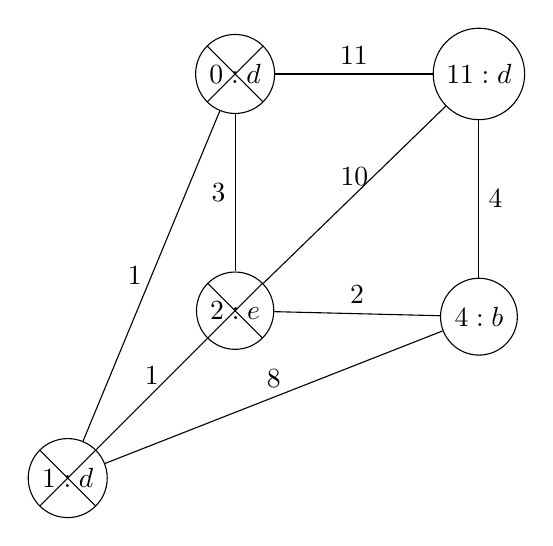
\begin{tikzpicture}
[cross/.style={path picture={ \draw[black] (path picture bounding
      box.south east) -- (path picture bounding box.north west) (path
      picture bounding box.south west) -- (path picture bounding
      box.north east); }}]
\node[draw,circle](a){$11:d$};
\node[draw,circle, below      =2cm of a](c){$4:b$};
\node[draw,circle,cross, left = 2cm of a](d){$0:d$};
\node[draw,circle,cross, below = 2 cm of d](b){$2:e$};
\node[draw,circle,cross, below left = 2 cm of b](e){$1:d$};
\path (a) edge node[above]{10} (b);
\path (a) edge node[right]{4} (c);
\path (b) edge node[left]{3} (d);
\path (a) edge node[above]{11} (d);
\path (b) edge node[above]{2} (c);
\path (b) edge node[above]{1} (e);
\path (d) edge node[left]{1} (e);
\path (c) edge node[above]{8} (e);
\end{tikzpicture}
\end{center}
Since the target node is the lowest available node the algorithm stops and, following back the route is $debc$.
\fi


\item In chess a knight moves three squares in one cardinal direction followed by one square in a perpendicular direction. In the chess board below the knight is in the bottom left-hand position, the two squares that it can reach in one move are marked \lq{}1\rq{}, what is the least number of moves that will take it to the square marked $\times$?
\begin{center}
%http://tex.stackexchange.com/questions/133332/to-draw-a-chessboard
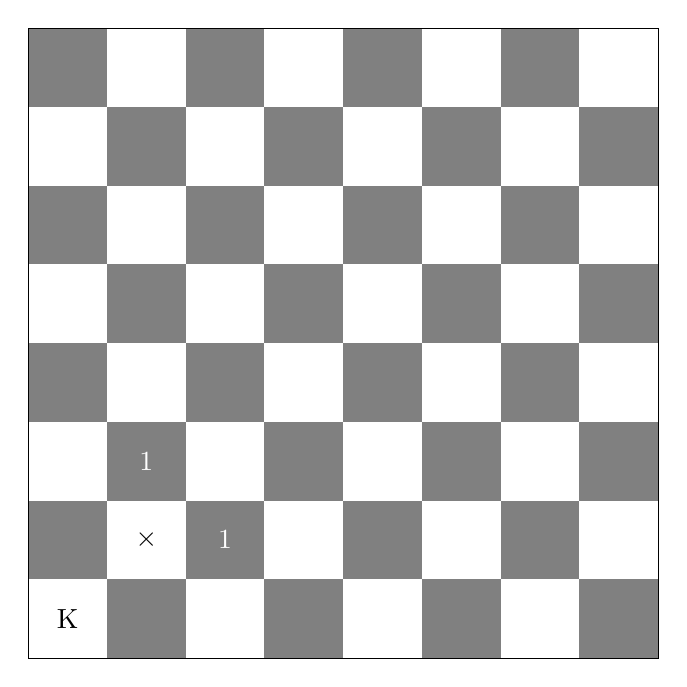
\begin{tikzpicture}[x=1cm]
    \foreach \x in {0,...,7} \foreach \y in {0,...,7}
    {
        \pgfmathparse{mod(\x+\y,2) ? "gray" : "white"}
        \edef\colour{\pgfmathresult}
        \path[fill=\colour] (\x,\y) rectangle ++ (1,1);
    }
    \draw (0,0)--(0,8)--(8,8)--(8,0)--cycle;

    \node at (.5, .5)(a) {K};
    \node at (1.5, 1.5)(a) {$\times$};
    \node[text = white] at (2.5, 1.5)(a) {1};
    \node[text = white] at (1.5, 2.5)(a) {1};

\end{tikzpicture}
\end{center}

\ifanswers


\noindent Solution:

This is just a version of Dijkstra's algorithm, do each node in turn and then cross if off, let's use a box to mark the crossed off nodes.
\begin{center}
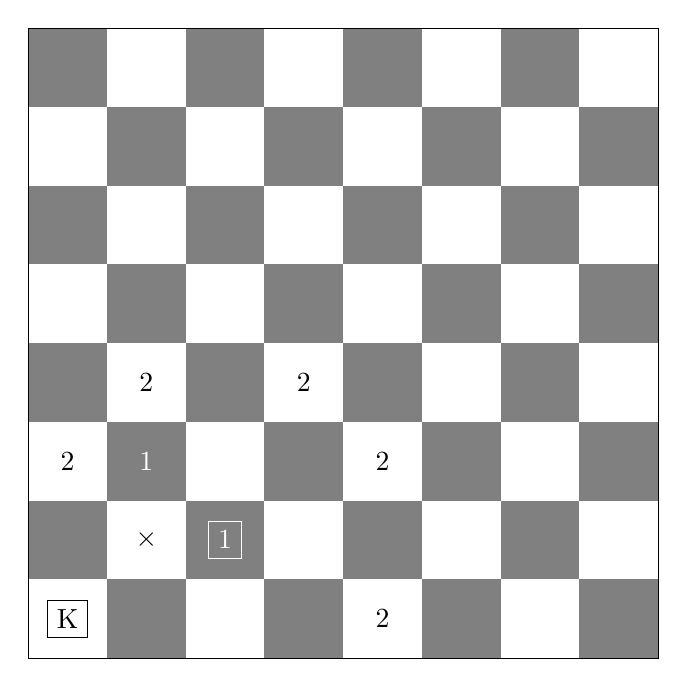
\begin{tikzpicture}[x=1cm]
    \foreach \x in {0,...,7} \foreach \y in {0,...,7}
    {
        \pgfmathparse{mod(\x+\y,2) ? "gray" : "white"}
        \edef\colour{\pgfmathresult}
        \path[fill=\colour] (\x,\y) rectangle ++ (1,1);
    }
    \draw (0,0)--(0,8)--(8,8)--(8,0)--cycle;
    \node at (1.5, 1.5)(a) {$\times$};
    \node[draw] at (.5, .5)(a) {K};
    \node[text = white,white,draw] at (2.5, 1.5)(a) {1};
    \node at (1.5, 3.5)(a) {2};
    \node at (3.5, 3.5)(a) {2};
    \node at (4.5, 2.5)(a) {2};
    \node at (4.5, 0.5)(a) {2};
    \node at (0.5, 2.5)(a) {2};

    \node[text = white] at (1.5, 2.5)(a) {1};

\end{tikzpicture}
\end{center}
Now all the \lq{}3\rq{} squares are going to be black, so the knight can't reach the $\times$ this go, so let's deal with all the \lq{}2\rq{} squares straight away. 
\begin{center}
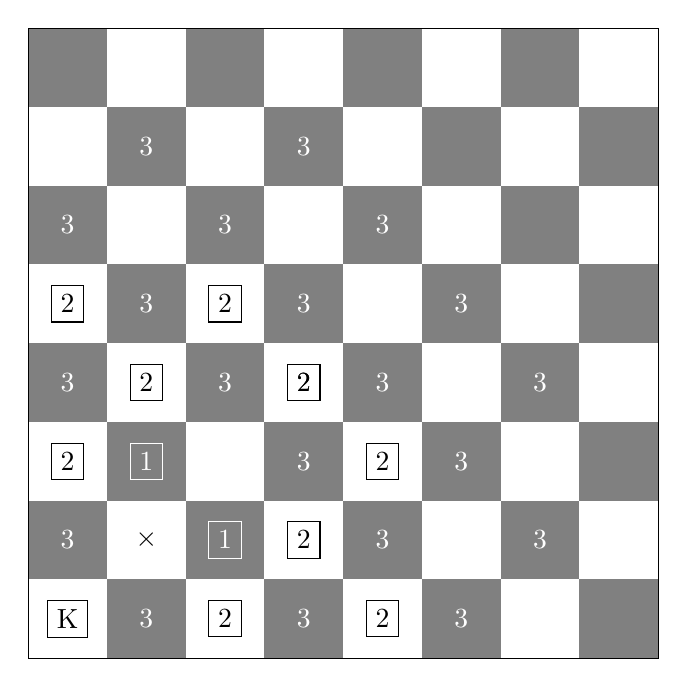
\begin{tikzpicture}[x=1cm]
    \foreach \x in {0,...,7} \foreach \y in {0,...,7}
    {
        \pgfmathparse{mod(\x+\y,2) ? "gray" : "white"}
        \edef\colour{\pgfmathresult}
        \path[fill=\colour] (\x,\y) rectangle ++ (1,1);
    }
    \draw (0,0)--(0,8)--(8,8)--(8,0)--cycle;
    \node at (1.5, 1.5)(a) {$\times$};
    \node[draw] at (.5, .5)(1) {K};
    \node[text = white,white,draw] at (2.5, 1.5)(2) {1};
    \node[draw] at (1.5, 3.5)(3) {2};
    \node[draw] at (3.5, 3.5)(4) {2};
    \node[draw] at (4.5, 2.5)(5) {2};
    \node[draw] at (4.5, 0.5)(6) {2};
    \node[draw] at (0.5, 2.5)(7) {2};

    \node[text = white,white,draw] at (1.5, 2.5)(8) {1};
    \node[draw] at (0.5, 4.5)(9) {2};
    \node[draw] at (2.5, 4.5)(10) {2};
    \node[draw] at (3.5, 3.5)(11) {2};
    \node[draw] at (3.5, 1.5)(12) {2};
    \node[draw] at (2.5, 0.5)(13) {2};

    \node[text = white] at (0.5, 1.5)(14) {3};
    \node[text = white] at (1.5, 0.5)(15) {3};
    \node[text = white] at (0.5, 3.5)(16) {3};
    \node[text = white] at (3.5, 0.5)(17) {3};
    \node[text = white] at (0.5, 5.5)(18) {3};
    \node[text = white] at (5.5, 0.5)(19) {3};
    \node[text = white] at (1.5, 4.5)(18) {3};
    \node[text = white] at (4.5, 1.5)(19) {3};
    \node[text = white] at (2.5, 3.5)(18) {3};
    \node[text = white] at (3.5, 2.5)(19) {3};

    \node[text = white] at (1.5, 6.5)(19) {3};
    \node[text = white] at (2.5, 5.5)(19) {3};
    \node[text = white] at (3.5, 4.5)(19) {3};
    \node[text = white] at (4.5, 3.5)(19) {3};
    \node[text = white] at (5.5, 2.5)(19) {3};
    \node[text = white] at (6.5, 1.5)(19) {3};

    \node[text = white] at (3.5, 6.5)(19) {3};
    \node[text = white] at (4.5, 5.5)(19) {3};
    \node[text = white] at (5.5, 4.5)(19) {3};
    \node[text = white] at (6.5, 3.5)(19) {3};

\end{tikzpicture}
\end{center}
The next move will reach the $\times$ so the answer is four.

\fi

\end{enumerate}

\end{document}
